\documentclass[11pt]{article}

%%%%%%%%%%%%%%%%%%%%%%%%
% Package Inclusion                                        
%%%%%%%%%%%%%%%%%%%%%%%%

\usepackage{amsmath} % Required for many math properties. AMS stands for American Mathematical Society.
\usepackage{amssymb} %Required for using many math symbols.
\usepackage{geometry} % Required for adjusting page dimensions.
\usepackage[utf8]{inputenc} % Required for inputting international characters.
\usepackage[none]{hyphenat} % Removes automatic hyphenation (a personal pet peeve of Sam).
\usepackage{hyperref} % Required to include URLs
\usepackage{xcolor} % Required to turn URLs the correct colors.
\usepackage{listings} % Required to display code.
\usepackage{bm} % Required to make vectors bold. 
\usepackage{graphicx}
\usepackage{float}
\usepackage{tikz}%Used for graph theory graphs
%%%%%%%%%%%%%%%%%%%%%%%%
% Page settings                                              
%%%%%%%%%%%%%%%%%%%%%%%%

% Set up page dimensions.
\geometry{
    paper=letterpaper, % 8.5 x 11 paper.
	top=1in, % Top margin.
	bottom=1in, % Bottom margin.
	left=1in, % Left margin.
	right=1in, % Right margin.
}
 % Set up code display settings
\lstset{
frame = single, % Box the code
numbers=left % Show line numbers
}
% Set up line and paragraph spacing
\setlength{\parindent}{0em} % Sets paragraph indentation
\setlength{\parskip}{1em} % Sets paragraph spacing
\linespread{1.0} % Sets line spacing

% Document attributes
\title{Research Project}
\author{Jonah Merrell}
\date{\today}

%%%%%%%%%%%%%%%%%%%%%%%%%%%%%%%%%%%%
% Begin the content which will be displayed in the output PDF
% Only things in between \begin{document} and \end{document} actually show up on your paper!
%%%%%%%%%%%%%%%%%%%%%%%%%%%%%%%%%%%%

\begin{document}
%\maketitle
\begin{flushright}
Jonah Merrell \\ 
\today \\
\end{flushright}

\begin{center}
{\LARGE Solving Systems of Non-Linear Differential Equations}
\end{center}

In order to solve a system of non-linear differential equations, we will implement various numerical methods. Consequently, the solutions generated will only be approximations, are subject to errors due to machine precision, and will not always be stable. However, the advantage of numerical methods is that they do not need to solve the solution analytically, which in many cases is not always possible.

In order to write a program capable of approximating a solution for a given system of differential equations, we will first tackle this problem by first breaking down the task into smaller, simpler tasks. We will build up to the system of non-linear differential equations solver with the following steps:
\begin{itemize}

\item Implement Euler's method to solve an orinary differential equation (EulerMethod)
\item Implement finite differences to solve more orinary differential equations 
\item Implement Euler's method to solve a partial differential equation (ODEeulerExplicit)
\item Implement Backwards Euler to solve a linear partial differential equation with greater stability (ODEeulerImplicit)
\item Implement Newtons method to solve a system of non-linear equations (NewtonMethodExample)
\item Implement Backwards Euler to solve a non-linear partial differential equation (ODEeulerImplicitNonLinear)
\item Implement Backwards Euler to solve a system non-linear partial differential equation \\ (ODEeulerImplicitNonLinearSystem3)
\end{itemize}

\newpage

\section*{Euler's method for an Ordinary Differential Equation}

Suppose we are given the following differential equation to solve:
\begin{align*}
    \frac{\partial y}{\partial x} = x*y + x + y
\end{align*}
One way to generate a solution for this differential equation over a certain interval is to use Euler's method. Euler's method works by recognizing that if we know $\frac{\partial y}{\partial x}$ and an initial condition $y(x_0) = y_0$, then we can approximate another point in the solution $y(x_1) = y_1$ with a linear approximation. Since we have a formula for $\frac{\partial y}{\partial x}$ , then we can approximate the next point in the solution by computing the following:

Given $(x_{j},y_{j})$, then $y_{j+1} = y_j + h*\frac{\partial y}{\partial x}$ and $x_{j+1} = x_j + h$. (Where $h$ is our step size. The smaller $h$ is, the more accurate our approximation for $y_{j+1}$).

Thus, by repeatedly computing $x_{j+1}$ and $y_{j+1}$ over an interval $[x_0,x_n]$, we generate a sequence of points $(x,y)$ that approximate solution for this differential equation within the interval.

Below shows an example of implementing Euler's method for the above differential equation
\begin{lstlisting}[language=Python]
import matplotlib.pyplot as plt

x_min = 0
x_max = 1.0
x_count = 50
dx = (x_max-x_min)/(x_count-1)
x_ = [x_min + j*dx for j in range(x_count)] #u[x][t]
x_[x_count-1] = x_max

y=[0 for i in range(x_count)]

def func(x, y):
    return (x + y + x * y) # dy / dx =(x + y + xy)
#apply initial condition y(0)
y[0] = 1.0
#Apply Euler's method
for j in range(x_count-1):
    y[j+1] = y[j] + dx * func(x_[j] , y[j])

#Everything below this is just for plotting y
plt.plot(x_,y,'r--', linewidth=2.0)
plt.xlabel("t")
plt.ylabel("S[N,C]")
plt.legend(["N","C"])
plt.show()
\end{lstlisting}

\newpage
\section*{Finite difference for Euler's method}
We now know how to apply Euler's method to a 1-dimensional ordinary differential equation, but so far we have only considered an example when $\frac{\partial y}{\partial x}$ was only dependant on $y$ and $x$. Suppose our differential equation involved multiple derivatives of $y$, such as the following example:
\begin{align*}
    \frac{\partial y}{\partial x} = x*y - \frac{\partial^{2} y}{\partial x^{2}}
\end{align*}
Euler's method requires us to compute $\frac{\partial y}{\partial x}$, but how can we compute $\frac{\partial y}{\partial x}$ if we do not yet know $\frac{\partial^{2} y}{\partial x^{2}}$? One way to work around this issue is to approximate $\frac{\partial y}{\partial x}$ and $\frac{\partial^{2} y}{\partial x^{2}}$ using finite difference approximations. 

The finite difference of $\frac{\partial y}{\partial x}$ is defined as:
\begin{align*}
\frac{\partial y_j}{\partial x_j} \approx \frac{y_{j+1}-y{j}}{\Delta x} \approx \frac{y_{j}-y_{j-1}}{\Delta x},
\end{align*}
and the finite difference for $\frac{\partial^{2} y}{\partial x^{2}}$ is define as:
\begin{align*}
\frac{\partial^{2} y_j}{\partial x_j^{2}} \approx \frac{y_{j+1}-2y_{j}+y_{j-1}}{\Delta x^2} \approx \frac{-y_{j-3}+4y_{j-2}-5y_{j-1}+2y_{j}}{\Delta x^2}
\end{align*}
These finite difference formulas come from the definition for the derivative.

Since we now know the finite difference for $\frac{\partial y}{\partial x}$ and $\frac{\partial^{2} y}{\partial x^{2}}$, we can replace them with their corresponding finite difference approximations in the differential equation. So as an example, we can now re-write our differential equation above as:
\begin{align*}
    \frac{y_{j+1}-y{j}}{\Delta x} = x_{j}*y_{j} - \frac{y_{j+1}-2y_{j}+y_{j-1}}{\Delta x^2}
\end{align*}
Now that we have equation defined in just terms of $x_j$, $y_j$, $y_{j-1}$, and $y_{j+1}$, we can rearrange the equation to solve for $y_{j+1}$. Then, in a manner similar to Euler's method, we can repeatedly compute $y_{j+1}$ over an interval $[x_0,x_n]$ to generate a sequence of points $(x,y)$ that approximate the solution for this differential equation.

As an example, re-arranging the equation above will produce:
\begin{align*}
    \frac{y_{j+1}-y{j}}{\Delta x} &= x_{j}*y_{j} - \frac{y_{j+1}-2y_{j}+y_{j-1}}{\Delta x^2}\\
    \frac{y_{j+1}}{\Delta x} - \frac{y_{j}}{\Delta x} &= x_{j}*y_{j} - \frac{y_{j+1}}{\Delta x^2} -\frac{-2y_{j}+y_{j-1}}{\Delta x^2}\\
    \frac{y_{j+1}}{\Delta x} +\frac{y_{j+1}}{\Delta x^2}&= \frac{y_{j}}{\Delta x} + x_{j}*y_{j} - \frac{-2y_{j}+y_{j-1}}{\Delta x^2}\\
    y_{j+1}*(\frac{1 + \Delta x}{\Delta x^2})&= \frac{y_{j}}{\Delta x} + x_{j}*y_{j} - \frac{-2y_{j}+y_{j-1}}{\Delta x^2}\\
    y_{j+1}&= (\frac{\Delta x^2}{1 + \Delta x}) (\frac{y_{j}}{\Delta x} + x_{j}*y_{j} - \frac{-2y_{j}+y_{j-1}}{\Delta x^2})\\
\end{align*}

Note: As with any second-order differential equation, we need 2 initial conditions $y(0)$ and $y'(0)$. This is needed in order to have enough information to know $y_{j-1}$ and $y_{j}$ to start the iteration. 

Final note: To obtain a more accurate approximation for $\frac{\partial^{2} y}{\partial x^{2}}$, you can use the right-sided finite difference approximation instead of the central-differnce approximation.



\newpage
\section*{Euler's method for a Partial Differential Equation}
Now that we know how to apply the Euler's method to a 1-dimensional ordinary differential equation (using finite differences), we are ready to consider how to implement it in multiple dimensions. Consider the following partial differential equation:
\begin{align*}
    \frac{\partial u}{\partial t} = D_u * \frac{\partial^{2} u}{\partial x^{2}}
\end{align*}
In this equation, $u$ is dependant on 2 independent variables $t$ and $x$. For this example, we will attempt to find a solution for $u$ only within a rectangular region of $t$ and $x$. Given the initial conditions, we can still use the finite difference to approximate another point in the solution. (Just like before in the 1-dimensional case). However, instead of just dealing with a single point as our initial condition $y(x_0) = y_0$, in multiple dimensions we must provide a function as our initial condition $u(x,0) = f(x)$. In addition, in multiple dimensions we must also deal with boundary conditions, which is the boundary of the rectangular region we are considering our solution on. The boundary conditions define the points on $u(x_0,t) = g(t)$ and $u(x_n,t) = h(t)$.

Like before, we can simply replace the differential terms in the equation above with their finite-difference equivalent.
\begin{align*}
    \frac{u^{n+1}_{j}-u^{n}_{j}}{\Delta t} = D_u * \frac{u^{n}_{j+1}-2u^{n}_{j}+u^{n}_{j-1}}{\Delta x^2}
\end{align*}
With the initial conditions $u(x,0) = f(x)$ and boundary conditions $u(x_0,t) = g(t)$ and $u(x_n,t) = h(t)$, it becomes straight-forward to re-arrange the equation to solve for $u^{n}_{j+1}$ and generate a solution.
\begin{align*}
    \frac{u^{n+1}_{j}-u^{n}_{j}}{\Delta t} = D_u * \frac{u^{n}_{j+1}-2u^{n}_{j}+u^{n}_{j-1}}{\Delta x^2}\\
    u^{n+1}_{j} - u^{n}_{j}= D_u *\Delta t*    \frac{u^{n}_{j+1}-2u^{n}_{j}+u^{n}_{j-1}}{\Delta x^2}\\
    u^{n+1}_{j} = u^{n}_{j} + D_u *\Delta t*    \frac{u^{n}_{j+1}-2u^{n}_{j}+u^{n}_{j-1}}{\Delta x^2}\\
\end{align*}

Below shows an example of implementing Euler's method for the above differential equation
\begin{lstlisting}[language=Python]
import numpy as np
import matplotlib.pyplot as plt
from mpl_toolkits import mplot3d
import math

Dv = 0.1 #a constant

x_min = 0.0
x_max = 1.0
x_count = 15 #15
dx = x_max/(x_count-1)
x_ = [x_min + j*dx for j in range(x_count)] #u[x][t]
x_[x_count-1] = x_max

t_min = 0.0
t_max = 2.0
t_count = 50 #50
dt = t_max/(t_count-1)
t_ =  [t_min + n*dt for n in range(t_count)] #u[x][t]
t_[t_count-1] = t_max

u=np.zeros((x_count,t_count))

#apply initial condition u(x,0) = f(x) on u
for j in range(x_count):
    u[j ,0] = math.sin(x_[j] * math.pi)

_lambda = (dt) / (dx ** 2)
for n in range(t_count-1):
    # Since our boundary conditions u(0,t) = 0 and u(1,t) = 0,
    #   I just leave them as zero
    for j in range(1, x_count - 1):
        u[j, n+1] = u[j,n] + Dv*_lambda*(u[j-1,n] - 2*u[j,n] + u[j+1,n])

#Everything below this is just for plotting u
x = np.linspace(x_min, x_max, x_count)
y = np.linspace(t_min, t_max, t_count)
X, Y = np.meshgrid(y, x)
fig = plt.figure()
ax = plt.axes(projection='3d')
ax.plot_wireframe(X, Y, u, color='grey')
ax.set_xlabel('t')
ax.set_ylabel('x')
ax.set_zlabel('z');
plt.show()
\end{lstlisting}

\newpage
\section*{Backwards Euler's method for a Linear Partial Differential Equation}
One of the issues that comes from solving a partial differential equation with Euler's method is stability. Initially, it would seem that our computation for $u^{n+1}_{j}$ increases in accuracy as the step size $\Delta x$ and $\Delta t$ approach zero, but this is only true to an extent. Eventually, decreasing $\Delta x$ and $\Delta t$ any further will cause the next iteration for $u^{n+1}_{j}$ to become unstable. This makes any additional computations for $u^{n+1}_{j}$ to be completely inaccurate.

In order to reduce this instability, we can implement the backwards Euler method, which is inherently more stable. (Also known as implicit Euler). Instead of approximating $\frac{\partial u_j}{\partial t_j}$ as $\frac{u_{j+1}-u{j}}{\Delta t}$ (the forward difference approximation), we can approximate $\frac{\partial u_j}{\partial t_j}$ as $\frac{u_{j}-u_{j-1}}{\Delta u}$ (the backward difference approximation).

Using our example from before, but using the backward difference approximation for $\frac{\partial u}{\partial t}$ instead, we get:
\begin{align*}
    \frac{\partial u}{\partial t} &= D_u * \frac{\partial^{2} u}{\partial x^{2}}\\
    \frac{u^{n}_{j}-u^{n-1}_{j}}{\Delta t} &= D_u * \frac{u^{n}_{j+1}-2u^{n}_{j}+u^{n}_{j-1}}{\Delta x^2}\\
    u^{n}_{j} - u^{n-1}_{j}&= D_u *\Delta t*    \frac{u^{n}_{j+1}-2u^{n}_{j}+u^{n}_{j-1}}{\Delta x^2}\\
    u^{n}_{j} &= u^{n-1}_{j} + D_u *\Delta t*    \frac{u^{n}_{j+1}-2u^{n}_{j}+u^{n}_{j-1}}{\Delta x^2}\\
    u^{n+1}_{j} &= u^{n}_{j} + D_u *\Delta t*    \frac{u^{n+1}_{j+1}-2u^{n+1}_{j}+u^{n+1}_{j-1}}{\Delta x^2}\\
\end{align*}
Before proceeding any further, we can already see that we can no longer solve for $u^{n+1}_{j}$ alone anymore, because $u^{n+1}_{j}$ is dependant on the variables $u^{n+1}_{j+1}$ and $u^{n+1}_{j-1}$, which we do not know. Attempting to solve for $u^{n+1}_{j+1}$ and $u^{n+1}_{j-1}$ in the same manner would only produce the equations:
\begin{align*}
    u^{n+1}_{j+1} &= u^{n}_{j+1} + D_u *\Delta t*    \frac{u^{n+1}_{j+2}-2u^{n+1}_{j+1}+u^{n+1}_{j}}{\Delta x^2}\\
    u^{n+1}_{j-1} &= u^{n}_{j-1} + D_u *\Delta t*    \frac{u^{n+1}_{j}-2u^{n+1}_{j-1}+u^{n+1}_{j-2}}{\Delta x^2}\\
\end{align*}
These additional equations still require knowing $u^{n+1}_{j-2}$ and $u^{n+1}_{j+2}$, and so we still haven't avoided the issue. This means that in order to solve for $u^{n+1}_{j}$, we must produce and then solve a system of equations, where $u^{n+1}_{1}$, $u^{n+1}_{2}$...$u^{n+1}_{x-2}$, $u^{n+1}_{x-1}$ are the unknowns. (The edges $u^{n+1}_{0}$ and $u^{n+1}_{x}$ are known, since they are defined from our boundary conditions)

If the partial differential equation is linear, then we can use linear algebra to solve the system of equations fairly easily. We can use the example differential equation above to demonstrate, since it is a linear differential equation. 

To solve a linear ordinary differential equation using backwards Euler, we first replace any instances of $\frac{\partial u}{\partial t}$ and $\frac{\partial^{2} u}{\partial t^{2}}$ with their corresponding finite difference approximation (as before), but using the backwards finite difference for $\frac{\partial u}{\partial t}$. Then, instead of solving for $u^{n+1}_{j}$, we solve for $u^{n}_{j}$ in terms of the unknowns $u^{n+1}_{j-1}$, $u^{n+1}_{j}$, and $u^{n+1}_{j+1}$. By doing this for each unknown $u^{n+1}_{1}$, $u^{n+1}_{2}$, $u^{n+1}_{3}$, ... $u^{n+1}_{x-1}$, we will obtain a system of linear equations of the form Ax = b.

Below shows an example:
\begin{align*}
    \frac{\partial u}{\partial t} &= D_u * \frac{\partial^{2} u}{\partial x^{2}}\\
    \frac{u^{n}_{j}-u^{n-1}_{j}}{\Delta t} &= D_u * \frac{u^{n}_{j+1}-2u^{n}_{j}+u^{n}_{j-1}}{\Delta x^2}\\
    \frac{u^{n+1}_{j}-u^{n}_{j}}{\Delta t} &= D_u * \frac{u^{n+1}_{j+1}-2u^{n+1}_{j}+u^{n+1}_{j-1}}{\Delta x^2}\\
    u^{n+1}_{j}-u^{n}_{j} &= D_u*\Delta t* \frac{u^{n+1}_{j+1}-2u^{n+1}_{j}+u^{n+1}_{j-1}}{\Delta x^2}\\
    -u^{n}_{j} &= -u^{n+1}_{j} +D_u*\Delta t* \frac{u^{n+1}_{j+1}-2u^{n+1}_{j}+u^{n+1}_{j-1}}{\Delta x^2}\\
    u^{n}_{j} &= u^{n+1}_{j} -D_u*\Delta t* \frac{u^{n+1}_{j+1}-2u^{n+1}_{j}+u^{n+1}_{j-1}}{\Delta x^2}\\
    u^{n}_{j} &= -\frac{D_u\Delta t}{\Delta x^2}*u^{n+1}_{j+1} + (1-2\frac{D_u\Delta t}{\Delta x^2})*u^{n+1}_{j} - \frac{D_u\Delta t}{\Delta x^2}*u^{n+1}_{j-1}
\end{align*}
For convinience, let $c = 1-2\frac{D_u\Delta t}{\Delta x^2}$ and $d=- \frac{D_u\Delta t}{\Delta x^2}$. Thus, we can write $u^{n}_{j}$ as:
\begin{align*}
    u^{n}_{j} &= d*u^{n+1}_{j+1} + c*u^{n+1}_{j} - d*u^{n+1}_{j-1}
\end{align*}

With this equation, we can generate the linear system Ax=b, where

$A = 
\left[ {\begin{array}{*{20}c}
   c & d & 0 & 0 & 0 & . & . & . & . & 0  \\
   d & c & d & 0 & 0 & . & . & . & . & 0  \\
   0 & d & c & d & 0 & . & . & . & . & 0  \\
   0 & 0 & d & c & d & . & . & . & . & 0  \\
   . & . & . & d & c & d & . & . & . & 0  \\
   . & . & . & . & d & c & d & . & . & 0  \\
   . & . & . & . & . & . & . & . & . & 0  \\
   . & . & . & . & . & . & d & c & d & 0  \\
   . & . & . & . & . & . & . & d & c & d  \\
   0 & 0 & 0 & 0 & 0 & 0 & 0 & 0 & d & c  \\
 \end{array} } \right]
$, $x = 
\left[ {\begin{array}{*{20}c}
   u^{n+1}_{1} \\
   u^{n+1}_{2} \\
   u^{n+1}_{3} \\
   u^{n+1}_{4} \\
   . \\
   . \\
   . \\
   . \\
   u^{n+1}_{x-2} \\
   u^{n+1}_{x-1} \\
 \end{array} } \right]
$, $b = 
\left[ {\begin{array}{*{20}c}
   u^{n}_{1} \\
   u^{n}_{2} \\
   u^{n}_{3} \\
   u^{n}_{4} \\
   . \\
   . \\
   . \\
   . \\
   u^{n}_{x-2} \\
   u^{n}_{x-1} \\
 \end{array} } \right]
$.

Now we can solve for x using any linear algebra solving technique (such as Gauss Elimination) to find the values for $u^{n+1}_{1}$, $u^{n+1}_{2}$, $u^{n+1}_{3}$, .... $u^{n+1}_{x-2}$, $u^{n+1}_{x-1}$.

Below shows an example of implementing the backwards Euler method for the above differential equation:

\begin{lstlisting}[language=Python]
import numpy as np
import matplotlib.pyplot as plt
from mpl_toolkits import mplot3d
import math

Dv = 0.1 #a constant

x_min = 0; x_max = 1.0; x_count = 50
dx = (x_max-x_min)/(x_count-1)
x_ = [x_min + j*dx for j in range(x_count)] #u[x][t]
x_[x_count-1] = x_max

t_min = 0.0; t_max = 2.0; t_count = 50
dt = (t_max-t_min)/(t_count-1)
t_ =  [t_min + n*dt for n in range(t_count)] #u[x][t]
t_[t_count-1] = t_max

u=np.zeros((x_count,t_count))
A=np.zeros((x_count,x_count))
#apply initial condition u(x,0) = f(x) on u
for j in range(x_count):
    u[j, 0] = math.sin(x_[j] * math.pi)

_lambda = (dt) / (dx ** 2)
for n in range(t_count-1):
    A[0,0] = 1
    A[x_count-1, x_count-1] = 1
    #Set up system of equations to solve for all values of j at n+1
    for j in range(1,x_count-1):
        #u[j, n + 1] = u[j,n] + Dv *_lambda * (u[j - 1,n] - 2*u[j,n] + u[j + 1,n]) #explicit solution
        A[j, j-1] = -Dv * _lambda
        A[j, j  ] = (1 + 2 * Dv * _lambda)
        A[j, j+1] = -Dv * _lambda

    #Solve for x given Ax = b
    u[:,n+1] = np.linalg.solve(A, u[:, n])

#Everything below this is just for plotting u
x = np.linspace(x_min, x_max, x_count)
y = np.linspace(t_min, t_max, t_count)
X, Y = np.meshgrid(y, x)
ax = plt.axes(projection='3d')
ax.plot_wireframe(X, Y, u, color='grey')
ax.set_xlabel('t')
ax.set_ylabel('x')
ax.set_zlabel('z');
plt.show()
\end{lstlisting}

\newpage
\section*{Newton's Method Applied to a System of Equations}

We have now successfully generated a solution for a linear partial differential equation using Euler's method. However, not all partial differential equations are linear. For example, consider the differential equation we have been using as our example before, but with one difference: 

\begin{align*}
    \frac{\partial u}{\partial t} = D_u * \frac{\partial^{2}}{\partial x^{2}}u^2
\end{align*}

Now, the above partial differential equation is no longer linear. Using forward Euler (or explicit Euler), it is still straightforward to solve for $u^{n+1}_{j}$ using the same methods as before:
\begin{align*}
    \frac{\partial u}{\partial t} &= D_u * \frac{\partial^{2}}{\partial x^{2}}u^2\\
    \frac{u^{n+1}_{j}-u^{n}_{j}}{\Delta t}&= D_u * \frac{(u^{n}_{j+1})^2-(2u^{n}_{j})^2+(u^{n}_{j-1})^2}{\Delta x^2}\\
    \frac{u^{n+1}_{j}-u^{n}_{j}}{\Delta t} &= D_u * \frac{(u^{n}_{j+1})^2-(2u^{n}_{j})^2+(u^{n}_{j-1})^2}{\Delta x^2}\\
    u^{n+1}_{j} - u^{n}_{j}&= D_u *\Delta t*    \frac{(u^{n}_{j+1})^2-(2u^{n}_{j})^2+(u^{n}_{j-1})^2}{\Delta x^2}\\
    u^{n+1}_{j} &= u^{n}_{j} + D_u *\Delta t*    \frac{(u^{n}_{j+1})^2-(2u^{n}_{j})^2+(u^{n}_{j-1})^2}{\Delta x^2}\\
\end{align*}
We can now generate a solution using Euler's method.

Unfortunately, backwards Euler is not as simple to implement. Attempting to implement backwards Euler as far as possible, we can still produce the equation:
\begin{align*}
    u^{n}_{j} &= -\frac{D_u\Delta t}{\Delta x^2}*(u^{n+1}_{j+1})^2 + (1-2\frac{D_u\Delta t}{\Delta x^2})*(u^{n+1}_{j})^2 - \frac{D_u\Delta t}{\Delta x^2}*(u^{n+1}_{j-1})^2
\end{align*}

But now, we can no longer rely on linear algebra to solve the resulting system of equations produced from this equation. We are still motivated to use backwards Euler because it is much more stable than forward Euler, which brings us to Newtons method.

Newton's method is an iterative method that can approximate the root of a non-linear equation. It works by taking an initial guess $x_0$, and recognizing that a more accurate root $x_{k+1} = x_0 - \frac{f(x_0)}{f'(x_0)}$. See the diagram below to help understand how Newton's method works

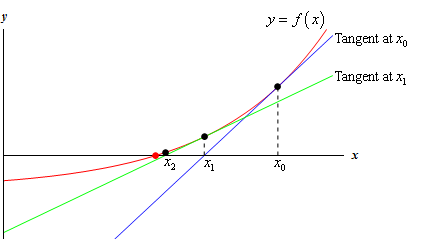
\includegraphics{NewtonsMethodImage.png}

By iterating the equation $x_{k+1} = x_{k} - \frac{f(x_{k})}{f'(x_{k})}$, we can find the root of the equation to a desired accuracy within machine precision.

Below shows an example of implementing Newton's method:

\begin{lstlisting}[language=Python]
import math
def f(x):
    return math.cos(x) - x
def f_prime(x):
    return -math.sin(x) - 1

x_0 = 1.0; x_1 = 1.1; tol = 0.000001; maxiter = 20; error = 10*tol; iter = 0
while(error > tol and iter < maxiter):
    iter += 1
    x_1 = x_0 - f(x_0) / f_prime(x_0)
    error = abs(x_1 - x_0)
    x_0 = x_1
print(x_1)
\end{lstlisting}

However, we still need to know how to implement Newton's method for a system of equations. In 1 dimension, the Newton iteration is $x_{k+1} = x_{k} - \frac{f(x_{k})}{f'(x_{k})}$. However, in multiple dimensions, we can no longer divide by the derivative, since we are dealing with multiple functions and multiple unknown variables, resulting in multiple derivatives. Instead, we compute the Jacobian matrix for the system of equations, which is essentially the multi-dimensional equivalent of the derivative. And since you can not divide by a matrix, we must either compute the inverse of the jacobian, or solve the system of equations using another method.
\\
The following shows the derivation for implementing Newton's method for a system of equations:
\begin{align*}
    x_{k+1} &= x_{k} - \frac{f(x_{k})}{f'(x_{k})}\\
    \implies x_{k+1} - x_{k} &= - \frac{f(x_{k})}{f'(x_{k})}\\
    \implies \Delta x &= - \frac{f(x_{k})}{f'(x_{k})}\\
    \implies f'(x_{k})*\Delta x &= - f(x_{k})\\
\end{align*}
Applied to a system of equations, this becomes:
\begin{align*}
    \implies J(u_{k})*\Delta u &= -F(u_{k})\\
\end{align*}
where 
$F = 
\left[ {\begin{array}{*{20}c}
   f_1(u) \\
   f_2(u) \\
   f_3(u) \\
   . \\
   . \\
 \end{array} } \right]
$, $J = 
\left[ {\begin{array}{*{20}c}
   \frac{\partial f_1}{\partial u^{n+1}_1} & \frac{\partial f_1}{\partial u^{n+1}_2} & \frac{\partial f_1}{\partial u^{n+1}_3} & . & .  \\
   \frac{\partial f_2}{\partial u^{n+1}_1} & \frac{\partial f_2}{\partial u^{n+1}_2} & \frac{\partial f_2}{\partial u^{n+1}_3} & . & .  \\
   \frac{\partial f_3}{\partial u^{n+1}_1} & \frac{\partial f_3}{\partial u^{n+1}_2} & \frac{\partial f_3}{\partial u^{n+1}_3} & . & .  \\
   . & . & . & . & . \\
   . & . & . & . & . \\
 \end{array} } \right]
$.

Since the system of equations is of the form Ax = b, we just solve the system of equations using a method such as Gauss Elimination to compute $\Delta u$. 
Then, to compute ${u^{n+1}_{j}}_{k+1}$ for the current iteration of Newtons method, we simply need to perform the following vector addition: $u_{k+1} = u_{k} + \Delta u$. We repeat this process for each iteration of Newton's method until we have achieved the desired accuracy.

Below shows a simple example of implementing Newton's method for a system of 2 equations with 2 unknowns.
\begin{lstlisting}[language=Python]
import numpy as np

#g=np.zeros((2,2))
J=np.zeros((2,2))
F=np.zeros(2)
u=np.zeros(2)
du=np.zeros(2)

u[0] = 1 #inital guess
u[1] = 2 #inital guess

for n in range(10):

    J[0,0] = 1
    J[0,1] = 2
    J[1,0] = 2*u[0]
    J[1,1] = 8*u[1]

    F[0] = u[0] + 2 * u[1] - 2  # = 0
    F[1] = u[0] ** 2 + 4 * u[1] ** 2 - 4  # = 0

    #The system of equations is J* dx = F
    du = np.linalg.solve(J, -F)
    u += du
print(u)
#Solution should be 0,1
\end{lstlisting}

\newpage
\section*{Backwards Euler applied to a Non-Linear Partial Differential Equation}

Now that we understand Newton's method, we can apply it to our backwards Euler method in order to solve a Non-Linear Partial Differential Equation. We will demonstrate this with an example:

Given the partial non-linear differential equation $\frac{\partial u}{\partial t} = D_u * \frac{\partial^{2}}{\partial x^{2}}u^2$, we can approximate it using the finite difference method. Then, we re-arrange the equation to form $F(u)=0$ for newton's method. Finally, we perform Newtons method to find the solution for $u^{n+1}_{j}$

\begin{align*}
    \frac{\partial u}{\partial t} &= D_u * \frac{\partial^{2}}{\partial x^{2}}u^2\\
    u^{n}_{j} &= -\frac{D_u\Delta t}{\Delta x^2}*(u^{n+1}_{j+1})^2 + (1-2\frac{D_u\Delta t}{\Delta x^2})*(u^{n+1}_{j})^2 - \frac{D_u\Delta t}{\Delta x^2}*(u^{n+1}_{j-1})^2\\
    f_j(u) = 0 &= -u^{n}_{j}-\frac{D_u\Delta t}{\Delta x^2}*(u^{n+1}_{j+1})^2 + (1-2\frac{D_u\Delta t}{\Delta x^2})*(u^{n+1}_{j})^2 - \frac{D_u\Delta t}{\Delta x^2}*(u^{n+1}_{j-1})^2 \\
\end{align*}

$F = 
\left[ {\begin{array}{*{20}c}
   f_1(u) \\
   f_2(u) \\
   f_3(u) \\
   . \\
   . \\
 \end{array} } \right]
$, $J = 
\left[ {\begin{array}{*{20}c}
   1+4\frac{D_u\Delta t}{\Delta x^2}*u^{n+1}_0 & -2\frac{D_u\Delta t}{\Delta x^2}*u^{n+1}_1 & 0 & . & . & . \\
   -2\frac{D_u\Delta t}{\Delta x^2}*u^{n+1}_0 & 1+4\frac{D_u\Delta t}{\Delta x^2}*u^{n+1}_1 & -2\frac{D_u\Delta t}{\Delta x^2}*u^{n+1}_2 & 0 & . & . \\
   0 & -2\frac{D_u\Delta t}{\Delta x^2}*u^{n+1}_1 & 1+4\frac{D_u\Delta t}{\Delta x^2}*u^{n+1}_2 & -2\frac{D_u\Delta t}{\Delta x^2}*u^{n+1}_1 & 0 & . \\
   0 & 0 & . & . & . & .\\
   . & . & . & . & . & .\\
   . & . & . & . & . & .\\
 \end{array} } \right]
$.

Finally, we solve the system $J(u_{k})*\Delta u = -F(u_{k})$ for $\Delta u$, and use $\Delta u$ to compute $u_{k+1} = u_{k} + \Delta u$. After repeating this for a few iterations, we will have an accurate approximation for $u_{k+1}$. Then, by iterating through Euler's method, we will obtain a solution in the region.
\begin{lstlisting}[language=Python]
import numpy as np
import matplotlib.pyplot as plt
from mpl_toolkits import mplot3d
import math

Dv = 0.1 #a constant

x_min = 0; x_max = 1.0; x_count = 50
dx = (x_max-x_min)/(x_count-1)
x_ = [x_min + j*dx for j in range(x_count)] #u[x][t]
x_[x_count-1] = x_max

t_min = 0.0; t_max = 2.0; t_count = 50
dt = (t_max-t_min)/(t_count-1)
t_ =  [t_min + n*dt for n in range(t_count)] #u[x][t]
t_[t_count-1] = t_max

u=np.zeros((x_count,t_count))
J=np.zeros((x_count,x_count))
F=np.zeros(x_count)
du=np.zeros(x_count-2)
#apply initial condition u(x,0) = f(x) on u
for j in range(x_count):
    u[j, 0] = math.sin(x_[j] * math.pi)
#Techniqually, we would now apply our boundary conditions on u here,
#    but since they're 0 in this case, there is no need.

_lambda = (dt) / (dx ** 2)
for n in range(t_count-1):
    u[:,n+1] = u[:,n] #Initial guess
    for i in range(10):
        #Set up jacobian matrix
        for j in range(1, x_count-1):#Remember, J is size x_count-2
            J[j, j-1] = -2*Dv * _lambda*u[j-1,n+1]
            J[j, j  ] = (1 + 4 * Dv * _lambda*u[j,n+1])
            J[j, j+1] = -2*Dv * _lambda*u[j+1,n+1]

        # Set up F Vector
        for j in range(1, x_count - 1):
            F[j] = u[j,n+1]-u[j, n] - Dv * _lambda*(u[j-1,n+1]**2 -
                2*u[j,n+1]**2 + u[j+1,n+1]**2)

        #Remove the boundry conditions columns/rows of J and F,
        #   since they are already known
        J_temp = np.delete(J, [0,x_count - 1], 0)
        J_temp = np.delete(J_temp, [0,x_count - 1], 1)
        F_temp = np.delete(F, [0,x_count - 1])

        #Solve the system J*du = -F for du (according to Newtons method)
        #   , then add du to u[:,n+1] to converge closer to solution
        du = np.linalg.solve(J_temp, -F_temp)
        u[:,n+1] += np.hstack([0, du, 0])#insert the boundry cond. rows 


#Everything below this is just for plotting u
x = np.linspace(x_min, x_max, x_count)
y = np.linspace(t_min, t_max, t_count)
X, Y = np.meshgrid(y, x)
fig = plt.figure()
ax = plt.axes(projection='3d')
ax.plot_wireframe(X, Y, u, color='grey')
ax.set_xlabel('t')
ax.set_ylabel('x')
ax.set_zlabel('z');
plt.show()
\end{lstlisting}

\newpage
\section*{Backward's Euler applied to a System of Non-Linear Partial Differential Equations}

To summarize what we have done so far, we can now solve a non-linear partial differential equation by utilizing backwards Euler and Newton's method. In order to do this, we break down the differential equation into a non-differential equation (using finite difference), and then approximate our solution by setting up a system of equations. The system of equations start from the initial and boundary conditions, and then approximate the rest of the solution (using Euler's method) within a specified region.

Solving a system of differential equations does not require any additional techniques than solving a single differential equation. First, we apply finite difference to each equation in the system. Then, we set up our system of equations involving $F(u)$ and $J(u)$ for Newton's method to solve for $u^{n+1}_j$ with our first equation. Then, we do the same thing for all the equations in the entire system of differential equations, to form a massive system of equations to solve. Newtons method and Euler's method will operate exactly the same.

Below shows an example:

Consider the System of equations:
\begin{align*}
    \frac{\partial u}{\partial t} &= D_u * \frac{\partial^{2}}{\partial x^{2}}u^2 + cuv\\
    \frac{\partial v}{\partial t} &= D_v * \frac{\partial^{2}v}{\partial x^{2}} + cuv
\end{align*}
Like before, we apply finite difference to the equations in the system, and then re-arrange them so that the left-hand side of the equation is 0. (In preparation for Newtons method).
\begin{align*}
    f_j(u) = 0 &= -u^{n}_{j}-\frac{D_u\Delta t}{\Delta x^2}*(u^{n+1}_{j+1})^2 + (1-2\frac{D_u\Delta t}{\Delta x^2})*(u^{n+1}_{j})^2 - \frac{D_u\Delta t}{\Delta x^2}*(u^{n+1}_{j-1})^2 + \Delta t*cuv\\
    f_j(v) = 0 &= -v^{n}_{j}-\frac{D_v\Delta t}{\Delta x^2}*v^{n+1}_{j+1} + (1-2\frac{D_v\Delta t}{\Delta x^2})*v^{n+1}_{j} - \frac{D_v\Delta t}{\Delta x^2}*v^{n+1}_{j-1} + \Delta t*cuv
\end{align*}

$F = 
\left[ {\begin{array}{*{20}c}
   f_1(u) \\
   f_2(u) \\
   f_3(u) \\
   . \\
   . \\
   f_1(v) \\
   f_2(v) \\
   f_3(v) \\
   . \\
   . \\
 \end{array} } \right]
$, $J = 
\left[ {\begin{array}{*{20}c}
   \frac{\partial f_1(u)}{\partial u^{n+1}_1} & \frac{\partial f_1(u)}{\partial u^{n+1}_2} & 0 & 0 & 0 & . & \frac{\partial f_1(u)}{\partial v^{n+1}_1} & 0 & 0 & 0 & 0 & .\\
   \frac{\partial f_2(u)}{\partial u^{n+1}_1} & \frac{\partial f_2(u)}{\partial u^{n+1}_2} & \frac{\partial f_2(u)}{\partial u^{n+1}_3} & 0 & 0 & . & 0 & \frac{\partial f_2(u)}{\partial v^{n+1}_2} & 0 & 0 & 0 & .\\
   0 & \frac{\partial f_3(u)}{\partial u^{n+1}_2} & \frac{\partial f_3(u)}{\partial u^{n+1}_3} & \frac{\partial f_3(u)}{\partial u^{n+1}_4} & 0 & . & 0 & 0 & \frac{\partial f_3(u)}{\partial v^{n+1}_3} & 0 & 0 & .\\
   0 & 0 & X & X & X & . & 0 & 0 & 0 & X & 0 & .\\
   0 & 0 & 0 & X & X & . & 0 & 0 & 0 & 0 & X & .\\
   . & . & . & . & . & . & . & . & . & . & . & .\\
   \frac{\partial f_1(v)}{\partial u^{n+1}_1} & 0 & 0 & 0 & 0 & . &\frac{\partial f_1(v)}{\partial v^{n+1}_1} & \frac{\partial f_1(v)}{\partial v^{n+1}_2} & 0 & 0 & 0 & .\\
   0 & \frac{\partial f_2(v)}{\partial u^{n+1}_2} & 0 & 0 & 0 & . & \frac{\partial f_2(v)}{\partial v^{n+1}_1} & \frac{\partial f_2(v)}{\partial v^{n+1}_2} & \frac{\partial f_2(v)}{\partial v^{n+1}_3} & 0 & 0 & .\\
   0 & 0 & \frac{\partial f_3(v)}{\partial u^{n+1}_3} & 0 & 0 & . & 0 & \frac{\partial f_3(v)}{\partial v^{n+1}_2} & \frac{\partial f_3(v)}{\partial v^{n+1}_3} & \frac{\partial f_3(v)}{\partial v^{n+1}_4} & 0 & .\\
   0 & 0 & 0 & X & 0 & . & 0 & 0 & X & X & X & .\\
   0 & 0 & 0 & 0 & X & . & 0 & 0 & 0 & X & X & .\\
   . & . & . & . & . & . & . & . & . & . & . & .\\
 \end{array} } \right]
$.

Using the Newton iteration as before, we solve the system $J(u_{k})*\Delta X = -F(u_{k})$ for $\Delta X$, and use $\Delta X$ to compute $X_{k+1} = X_{k} + \Delta X$. $X_{k+1}$ will contain the solutions for $u^{n+1}_{j}$ and $v^{n+1}_{j}$ in the following form:

$X_{k+1} = 
\left[ {\begin{array}{*{20}c}
   u^{n+1}_{1} \\
   u^{n+1}_{2} \\
   u^{n+1}_{3} \\
   . \\
   . \\
   v^{n+1}_{1} \\
   v^{n+1}_{2} \\
   v^{n+1}_{3} \\
   . \\
   . \\
 \end{array} } \right]
$.

After repeating this for a few iterations, we will have accurate approximations for $u^{n+1}_{j}$ and $v^{n+1}_{j}$. Then, by iterating through Euler's method, we will obtain a solution in the region.

\begin{lstlisting}[language=Python]
import numpy as np
import matplotlib.pyplot as plt
from mpl_toolkits import mplot3d
import math

#Solves a system of differential equations, where both equations depend
#   on the other. (we solve for them both simultaneously).

Du = 0.1 #a constant
Dv = 0.1 #a constant
c = 1.4 # a constant

x_min = 0; x_max = 1.0; x_count = 50
dx = (x_max-x_min)/(x_count-1)
x_ = [x_min + j*dx for j in range(x_count)] #u[x][t]
x_[x_count-1] = x_max

t_min = 0.0; t_max = 5.0; t_count = 50
dt = (t_max-t_min)/(t_count-1)
t_ =  [t_min + n*dt for n in range(t_count)] #u[x][t]
t_[t_count-1] = t_max

#Set up the inital variables
u=np.zeros((x_count,t_count))
v=np.zeros((x_count,t_count))
J=np.zeros((x_count*2,x_count*2))
F=np.zeros(x_count*2)


du=np.zeros(x_count)
dv=np.zeros(x_count)
#apply initial condition u(x,0) = f(x) on u
for j in range(x_count):
    u[j, 0] = math.sin(x_[j] * math.pi)
    v[j, 0] = 0.5*math.sin(x_[j] * math.pi)

_lambda = (dt) / (dx ** 2)

for n in range(t_count-1):

    u[:,n+1] = u[:,n] #Initial guess
    v[:, n + 1] = v[:, n]  # Initial guess
    for i in range(10):
        #Set up jacobian matrix for u
        for j in range(1,x_count-1):
            j2 = x_count+j
            J[j, j-1] = -2*Du * _lambda*u[j-1,n+1]
            J[j, j ] = 1 + 4 * Du * _lambda*u[j,n+1] - dt*c*v[j,n+1]
            J[j, j+1] = -2*Du * _lambda*u[j+1,n+1]

            J[j, j2] = -dt*c*u[j,n+1]

            J[j2, j2 - 1] = -1 * Dv * _lambda
            J[j2, j2] = 1 + 2 * Dv * _lambda - dt*c*u[j,n+1]
            J[j2, j2 + 1] = -1 * Dv * _lambda

            J[j2, j] = -dt*c*v[j, n + 1]

        # Set up F Vector for entire system.
        for j in range(1, x_count - 1):
            F[j] = u[j,n+1] - u[j, n] - Du*_lambda*(u[j-1,n+1]**2 -
                2*u[j,n+1]**2 + u[j+1,n+1]**2) - dt*c*u[j,n+1]*v[j,n+1]
            F[x_count + j] = v[j,n+1] - v[j,n] - Dv*_lambda*(v[j-1,n+1]
                - 2*v[j,n+1] + v[j+1,n+1]) - dt*c*u[j,n+1]*v[j,n+1]

        # Remove the boundry conditions columns/rows of J and F, 
        #   since they are already known
        J_temp = np.delete(J, [0, x_count - 1,x_count,2*x_count-1], 0)
        J_temp = np.delete(J_temp, [0, x_count - 1,x_count,2*x_count-1], 1)
        F_temp = np.delete(F, [0, x_count - 1,x_count,2*x_count-1])


        #Solve the system J*du = -F for du (according to Newtons method)
        #   , then add du to u[:,n+1] to converge closer to solution
        du = np.linalg.solve(J_temp, -F_temp)
        l = len(du)//2

        u[:,n+1] += np.hstack([0, du[:l], 0])
        v[:,n+1] += np.hstack([0, du[l:], 0])

#Everything below this is just for plotting u and v
x = np.linspace(x_min, x_max, x_count)
y = np.linspace(t_min, t_max, t_count)
X, Y = np.meshgrid(y, x)
fig = plt.figure()
ax = plt.axes(projection='3d')
ax.plot_wireframe(X, Y, u, color='grey')
ax.plot_wireframe(X, Y, v, color='red')
ax.set_xlabel('t')
ax.set_ylabel('x')
ax.set_zlabel('z');
plt.show()
\end{lstlisting}



\end{document}

